\documentclass[10pt,a4paper]{article}
\usepackage[utf8]{inputenc}
\usepackage[english]{babel}
\usepackage{amsmath}
\usepackage{amsfonts}
\usepackage{amssymb}
\usepackage{graphicx}
\usepackage{indentfirst}
\usepackage{fancyvrb}
\usepackage{subfigure}
\usepackage[shortlabels]{enumitem}
\usepackage[hidelinks]{hyperref}
\author{Giuseppe L'Erario}
\date{}
\title{K-Nearest Neighbours}

\begin{document}
\maketitle

\section*{Introduction}
	The \emph{K-Nearest Neighbours} is one of the simplest machine learning algorithms, particularly useful in pattern recognition. It is called \emph{lazy} algorithm, because it does not learn a function from train dataset, but instead learns it. 
	
	In this report is analysed a classification problem on a the famous \emph{Iris Dataset}.
	
\section*{Implementation}
	The KNN algorithm can be summarized in few steps:
		\begin{enumerate}[leftmargin=3\parindent]
			\item Choose the number \emph{k} of the neighbours;
			\item Choose a weight function;
			\item Find the k-nearest neighbours of the object to classify;
			\item Assign the label based on majority vote.
		\end{enumerate}
	
	The KKN algorithm finds the most similar \emph{k} samples in training dataset to the object to classify. This similarity is determined by the weight function. \\ 
	\\ The weight function used in this homework are:
	\begin{description}
		\item[Uniform]: all points in each neighbourhood are equally weighted;
		\item[Distance]: points are weighted with the inverse of the distance. Points closer to the query point have greater influence than further points;
		\item[Custom]: a gaussian function in the form $w=e^{-\alpha d^2}$, non-linearly dependent from the inverse of the distance. 
	\end{description}
	
	As usual the dataset is preprocessed and then reduced in dimensionality with PCA.
	
	The variation of the decision boundaries can be seen in fig.\ref{k_neighbors}. The core of the problem is to find the right number of the neighbors. A small \emph{k} leads to a classification linked too much with the single sample (in other words, to much sensible to outliers). With the increasing of \emph{k} the decision boundaries become smoother. They are, indeed, more dependant from a group of samples. A too high \emph{k} could lead to a too generalized classification: the algorithm will consider samples that are too distant, and probably are uncorrelated, from the query point.
	
	\begin{figure*}[hp]
		%\centering
		\subfigure[k = 1\label{k1}]{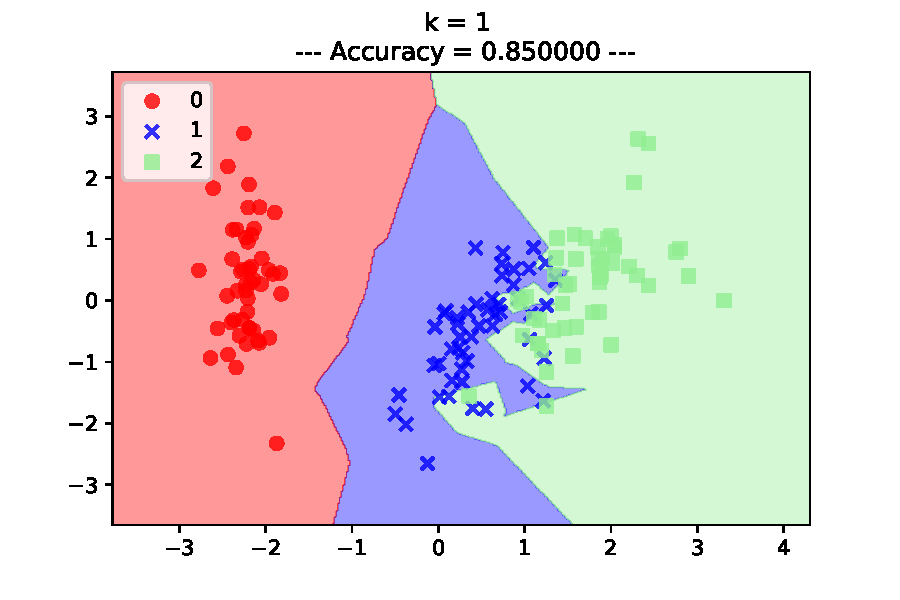
\includegraphics[width=0.4\linewidth]{../Images/k_1.pdf}}\qquad\qquad
		\subfigure[k = 2\label{k2}]{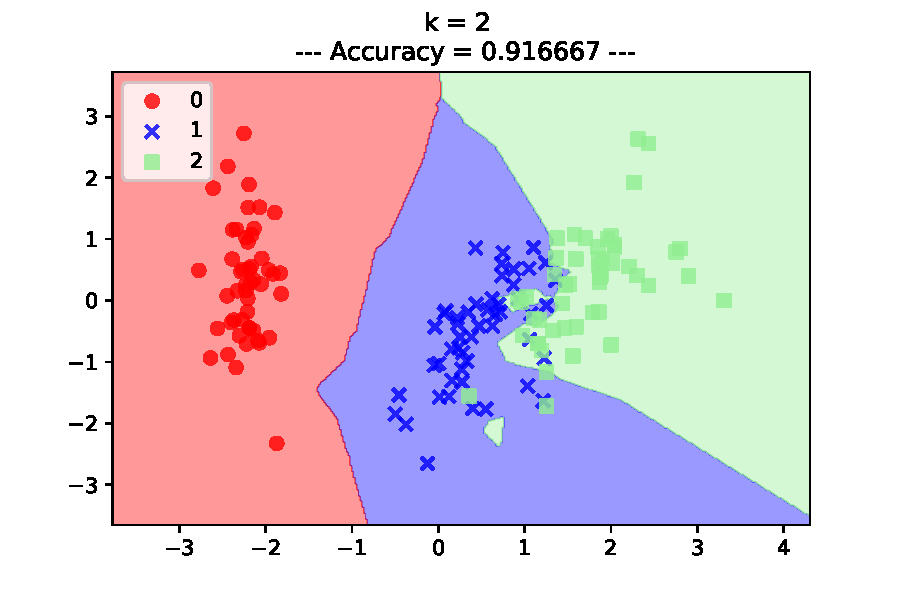
\includegraphics[width=0.4\linewidth]{../Images/k_2.pdf}}\qquad\qquad
		\subfigure[k = 3\label{k3}]{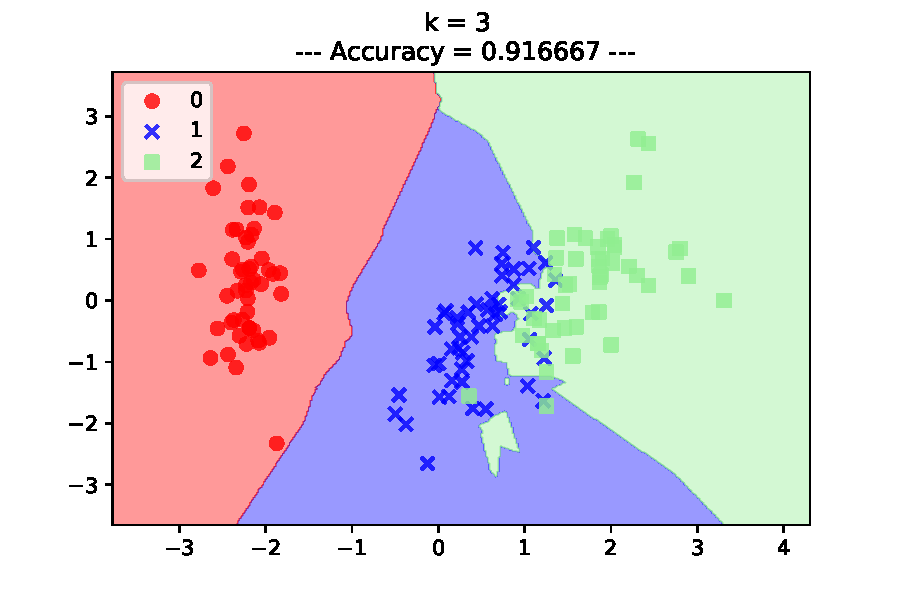
\includegraphics[width=0.4\linewidth]{../Images/k_3.pdf}}\qquad\qquad
		\subfigure[k = 4\label{k4}]{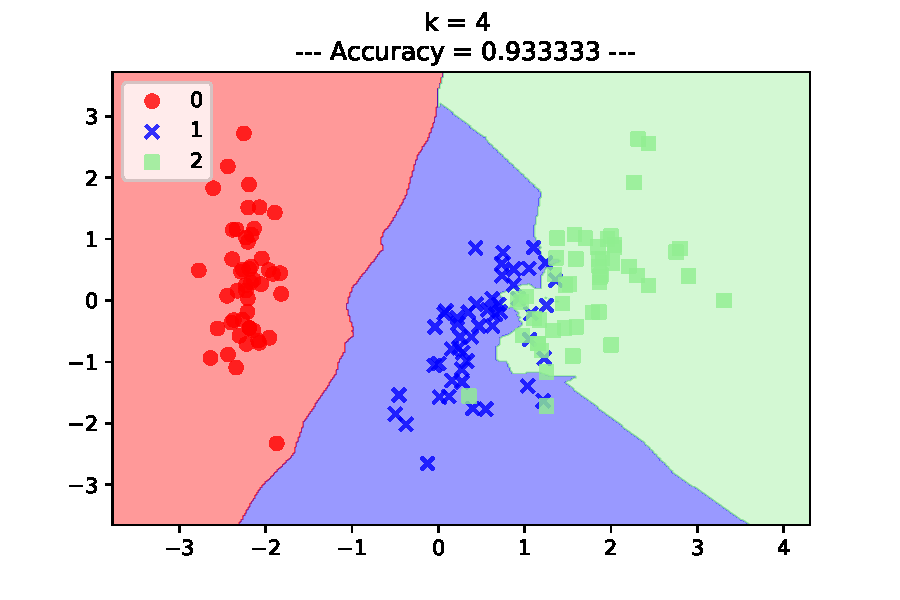
\includegraphics[width=0.4\linewidth]{../Images/k_4.pdf}}\qquad\qquad
		\subfigure[k = 5\label{k5}]{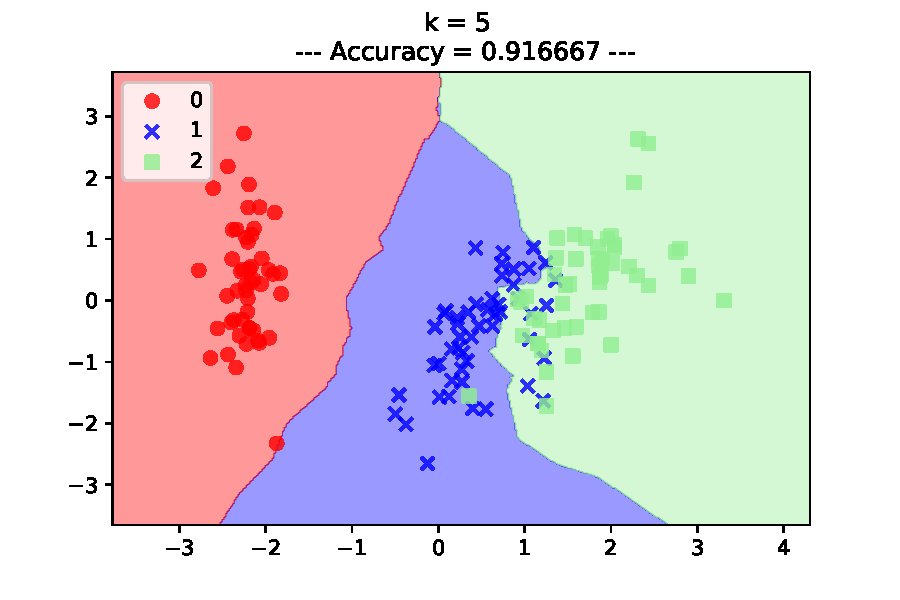
\includegraphics[width=0.4\linewidth]{../Images/k_5.pdf}}\qquad\qquad
		\subfigure[k = 6\label{k6}]{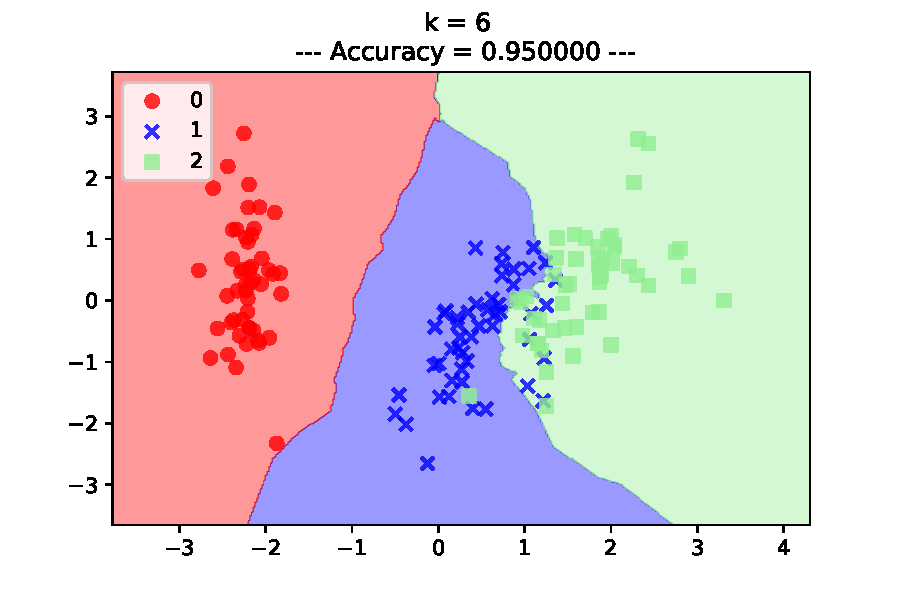
\includegraphics[width=0.4\linewidth]{../Images/k_6.pdf}}\qquad\qquad
		\subfigure[k = 7\label{k7}]{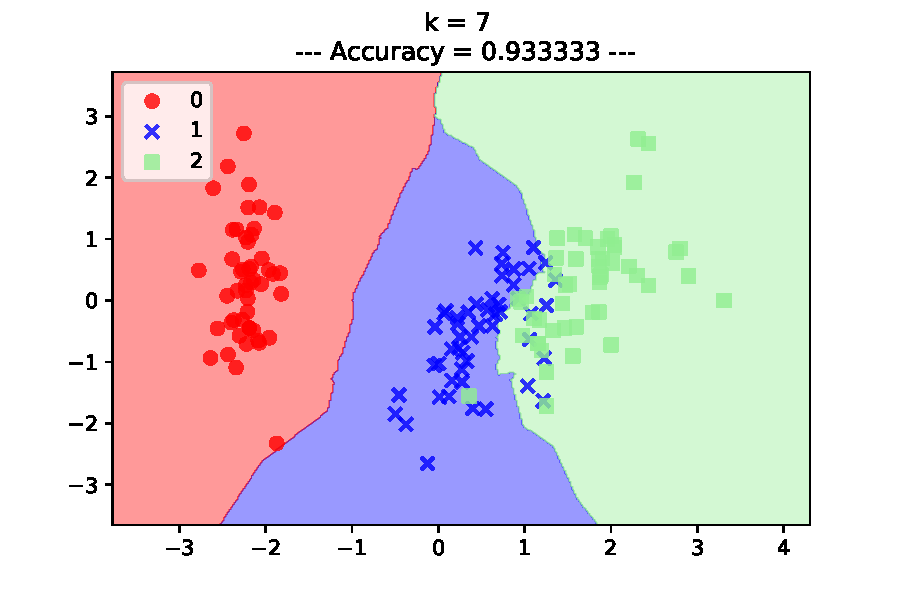
\includegraphics[width=0.4\linewidth]{../Images/k_7.pdf}}\qquad\qquad
		\subfigure[k = 8\label{k8}]{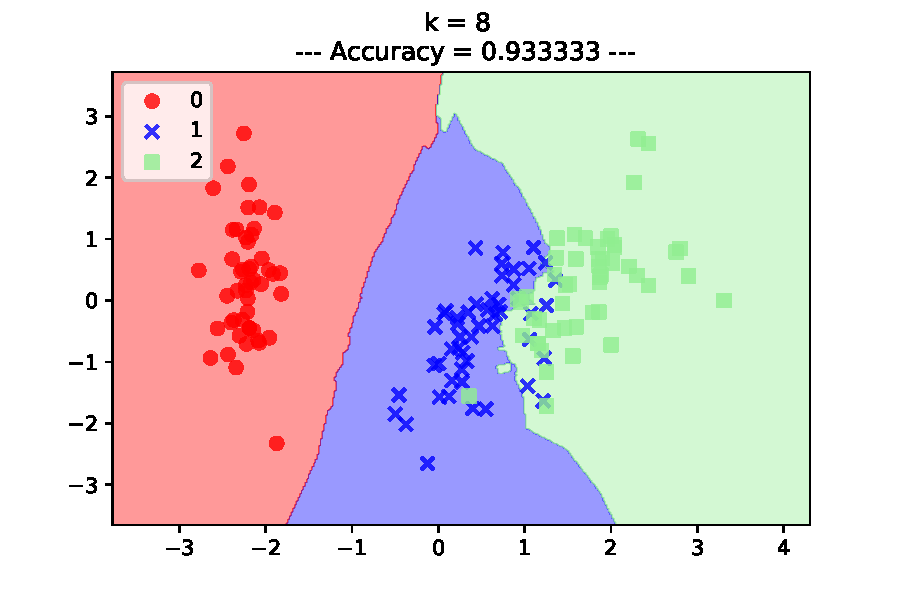
\includegraphics[width=0.4\linewidth]{../Images/k_8.pdf}}\qquad\qquad
		\subfigure[k = 9\label{k9}]{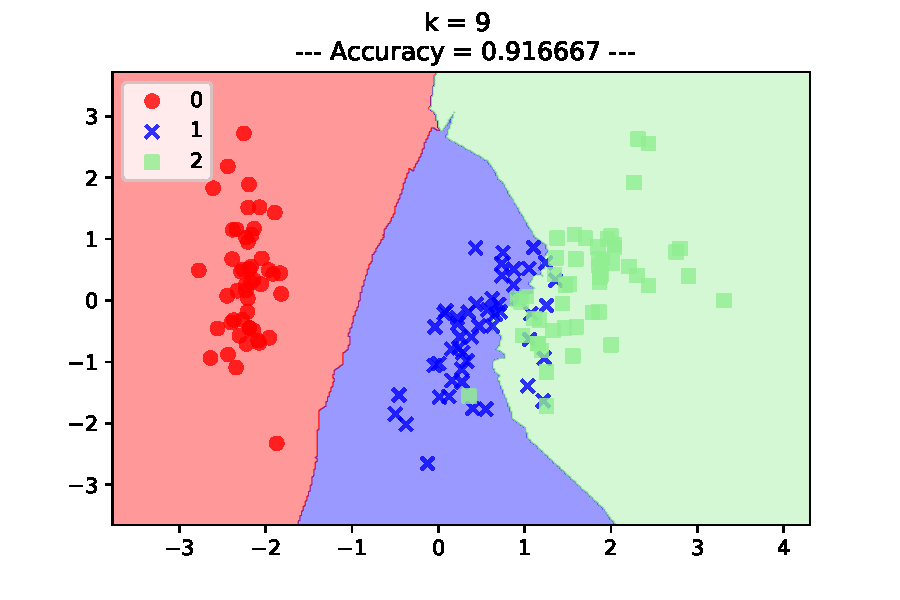
\includegraphics[width=0.4\linewidth]{../Images/k_9.pdf}}\qquad\qquad
		\subfigure[k = 10\label{k10}]{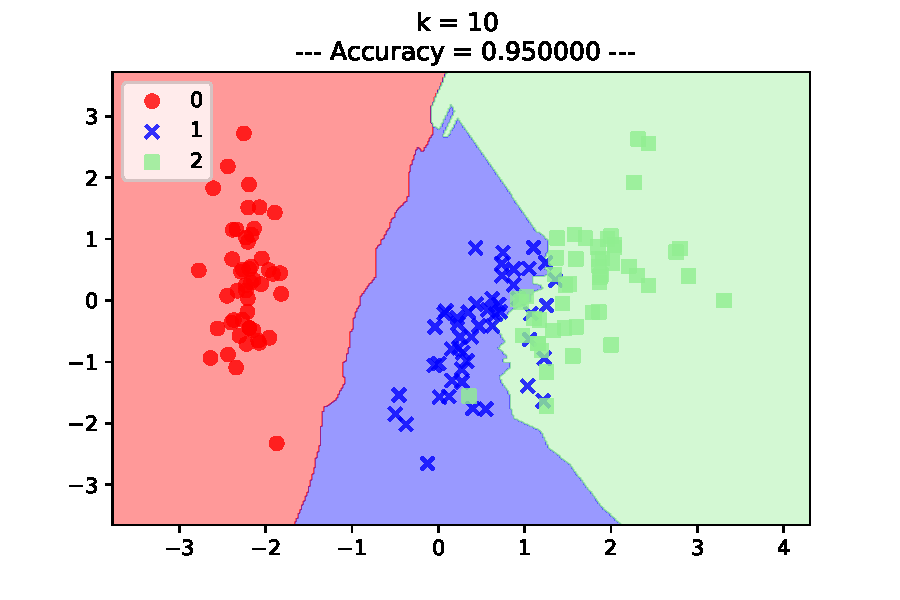
\includegraphics[width=0.4\linewidth]{../Images/k_10.pdf}}\qquad\qquad
		\caption{Variation of decision boundaries with the number of neighbors\label{k_neighbors}}
	\end{figure*} 
	
	\newpage
	

	
	For $k=3$ neighbors are used the \emph{'uniform} and \emph{'distance'} weight function (fig.\ref{weight_fun}). The accuracy is the same.
	
	\begin{figure}[hp]
		\centering
		\subfigure[Uniform]{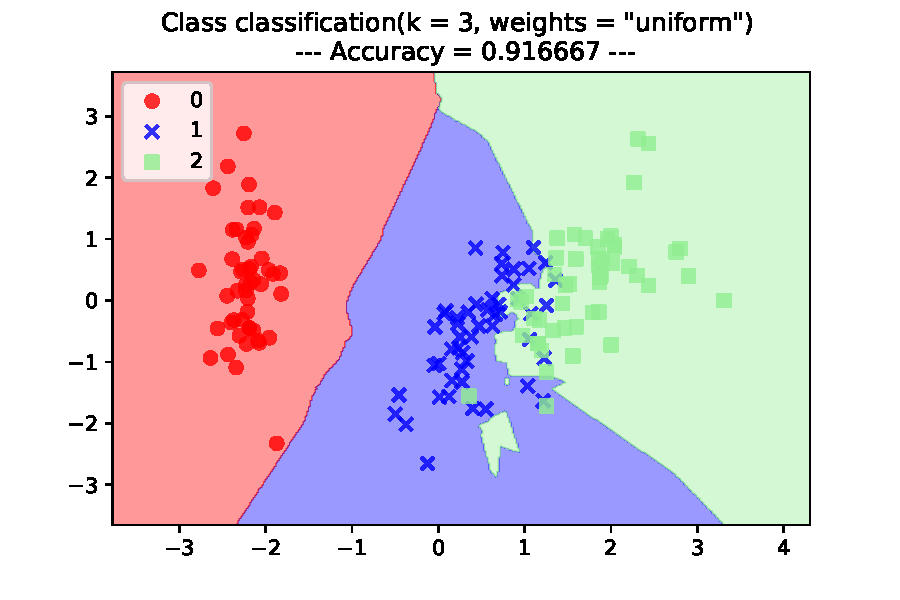
\includegraphics[width=0.4\linewidth]{../Images/k3_uniform.pdf}}\qquad\qquad
		\subfigure[Distance]{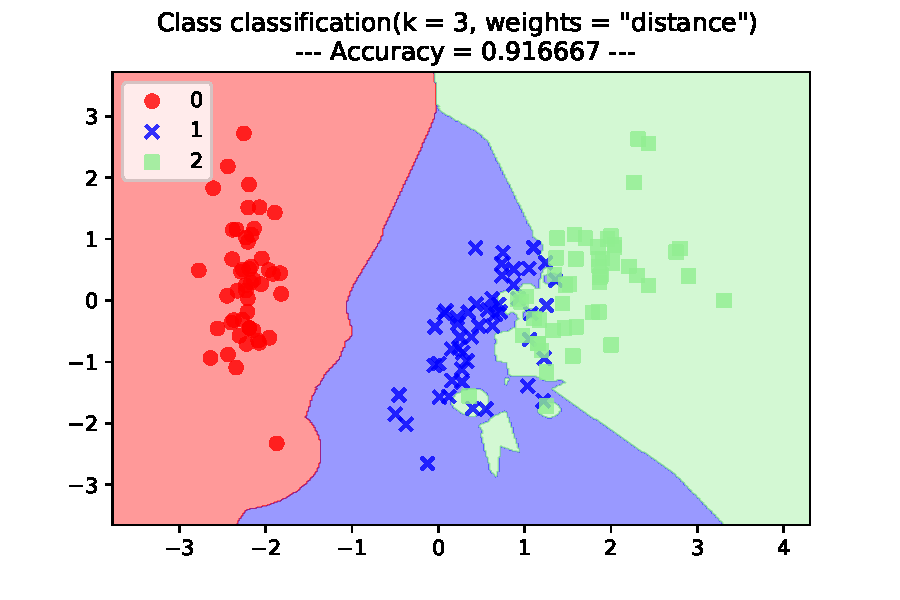
\includegraphics[width=0.4\linewidth]{../Images/k3_distance.pdf}}
		\caption{Weight functions\label{weight_fun}}
	\end{figure}
	
		In fig.\ref{fig:Accuracy_k} can be seen that the accuracy wrt. the number \emph{k}.
		
		\begin{figure}[hp]
			\centering
			\quad\subfigure[Uniform weight function]{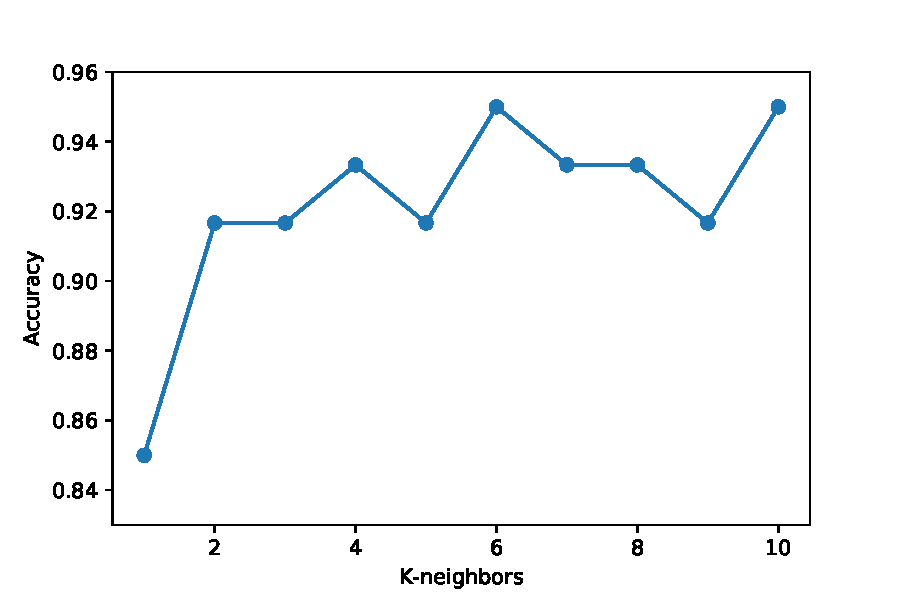
\includegraphics[width=0.4\linewidth]{../Images/Accuracy_k}}\qquad\qquad
			\subfigure[Distance weight function]{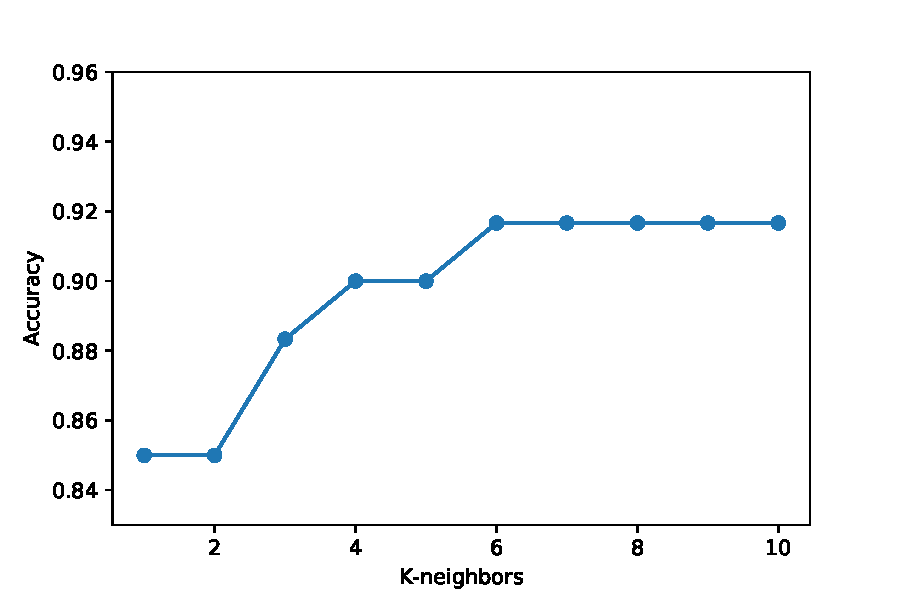
\includegraphics[width=0.4\linewidth]{../Images/Accuracy_k_distance}}\qquad\qquad
			\caption{Accuracy with the number of neighbors}
			\label{fig:Accuracy_k}
		\end{figure}
		
		\subsubsection*{Gaussian weight function}
		With a custom weight function we can tune how much the distance parameter is important in the classification problem, making this weight function more versatile. With the increasing of $\alpha$, the distance parameter is more and more important.
		
		In fig.\ref{gaussian} are plotted the decision boundaries, for $k=7$, on varying of $\alpha$. In correspondence of $\alpha=1000$ the fig.\ref{alpha1000} shows a visible difference in the decision boundaries. With huge values of $\alpha$ the weight function comes to zero quickly: the "influence zone" of the samples \emph{1} and \emph{2} becomes smaller\footnote{Probably the red zone, relative to \emph{0} group, is the last zone drawed}, only the closer samples are classified as belonging to the same class.
		
		\begin{figure}[!h]
			\centering
			\subfigure[$\alpha=0.1$\label{alpha0.1}]{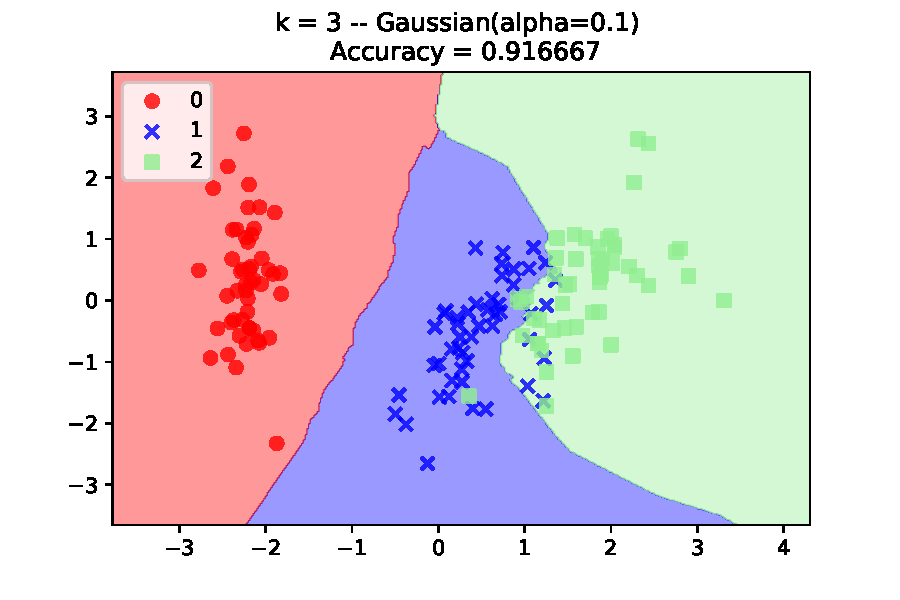
\includegraphics[width=0.4\linewidth]{../Images/alpha_01}}\qquad\qquad
			\subfigure[$\alpha=10$\label{alpha10}]{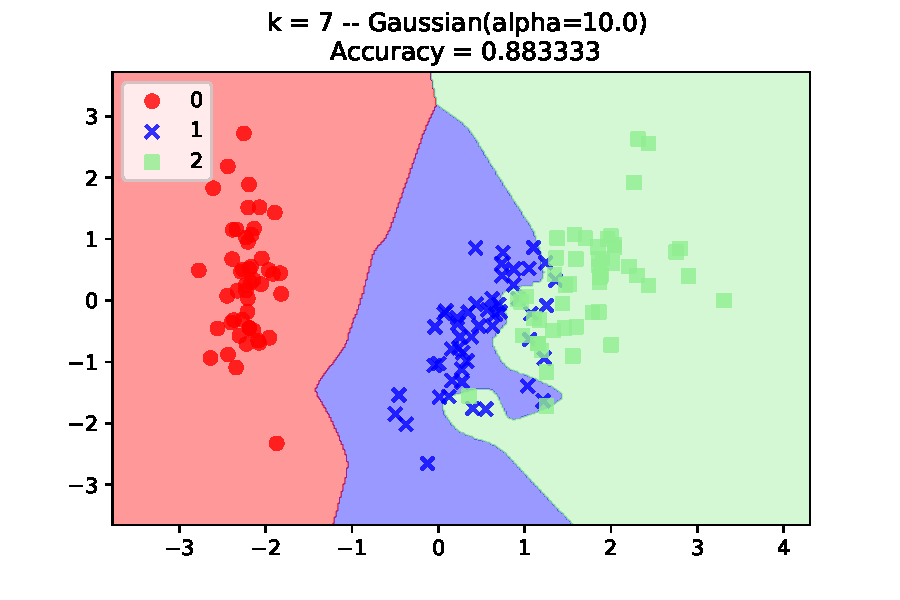
\includegraphics[width=0.4\linewidth]{../Images/alpha_10.pdf}}\qquad\qquad
			\subfigure[$\alpha=100$\label{alpha100}]{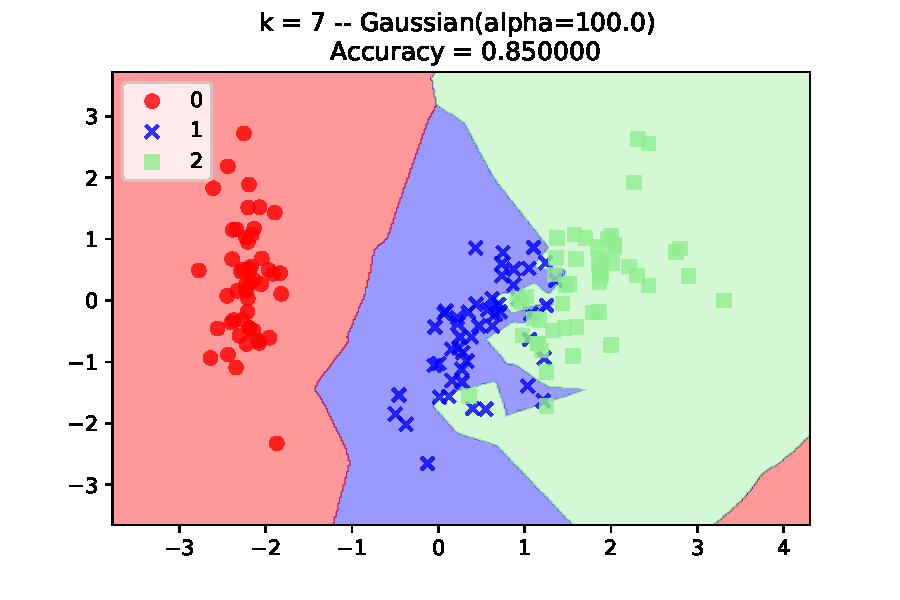
\includegraphics[width=0.4\linewidth]{../Images/alpha_100.pdf}}\qquad\qquad
			\subfigure[$\alpha=1000$\label{alpha1000}]{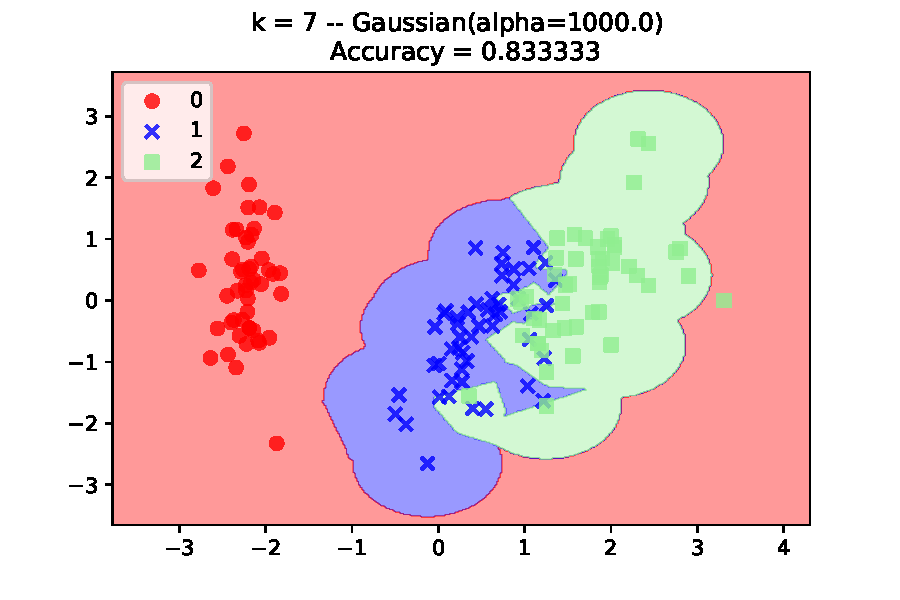
\includegraphics[width=0.4\linewidth]{../Images/alpha_1000.pdf}}
			\caption{Gaussian weight functions\label{gaussian}}
		\end{figure}
		
		In fig.\ref{fig:Accuracy_gaussian} is plotted the accuracy on varying of $\alpha$: the best performance are obtained with low value of $\alpha$.
		
		\begin{figure}[!h]
		\centering
		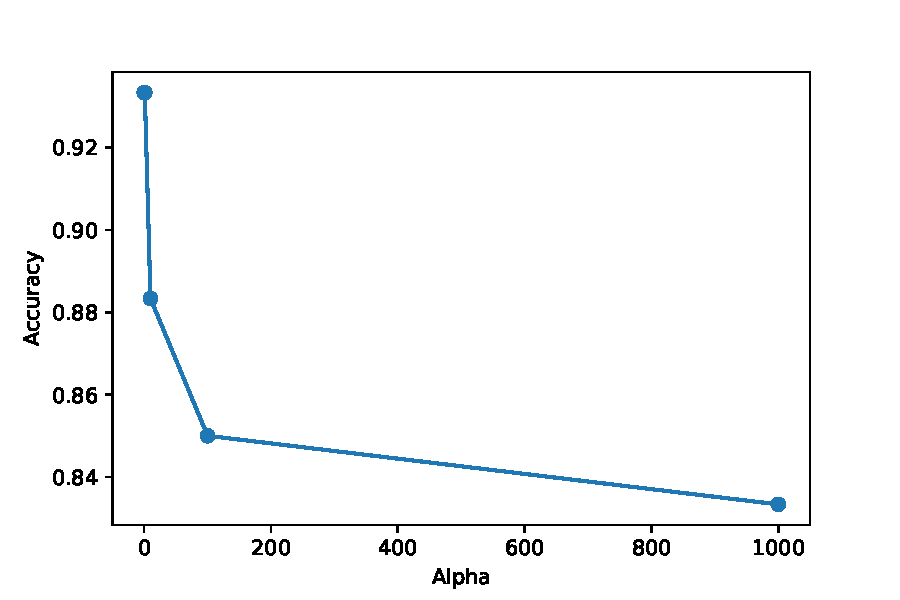
\includegraphics[width=0.7\linewidth]{../Images/Accuracy_gaussian}
		\caption{Accuracy on varying of $\alpha$.}
		\label{fig:Accuracy_gaussian}
		\end{figure}
		
		\newpage
		\subsubsection*{Best model}
		
		We can find the best model with a grid search, including number \emph{k} of neighbors, weight functions and $\alpha$ (using gaussian weight function).
		
		The model with the best performance is the one shown in fig.\ref{fig:Best_choice}.
		
		However, there is not a univocal best model with a precise weight function. In fact, it can be different from one simulation to another (due to the necessary random split of the data), or, in the same simulation, there also can be models with the same accuracy score. The shape of the boundaries are often very similar between the models. 
		
		For example, after a different simulation comes out that the best model is one with a gaussian weight function (fig.\ref{fig:Best_choice_Gaussian(alpha=1)}), but clearly leads to a misclassification of class \emph{0}.
		
		The only way to find a good model is to measure its accuracy, trying not to fall in overfitting issues.
		
		\begin{figure}[!ht]
		\centering
		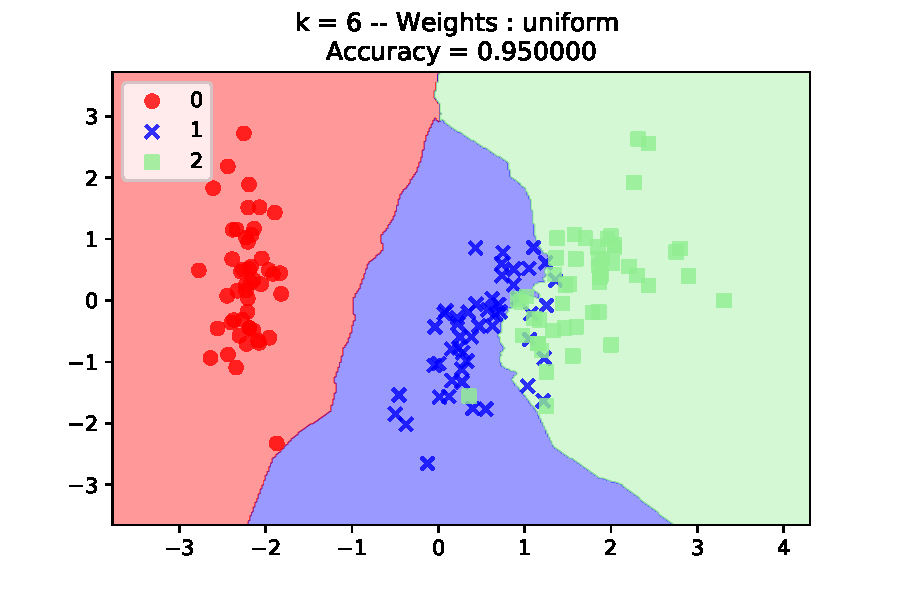
\includegraphics[width=0.7\linewidth]{../Images/Best_choice_uniform}
		\caption{Best model.}
		\label{fig:Best_choice}
		\end{figure}
		
		\begin{figure}[h]
		\centering
		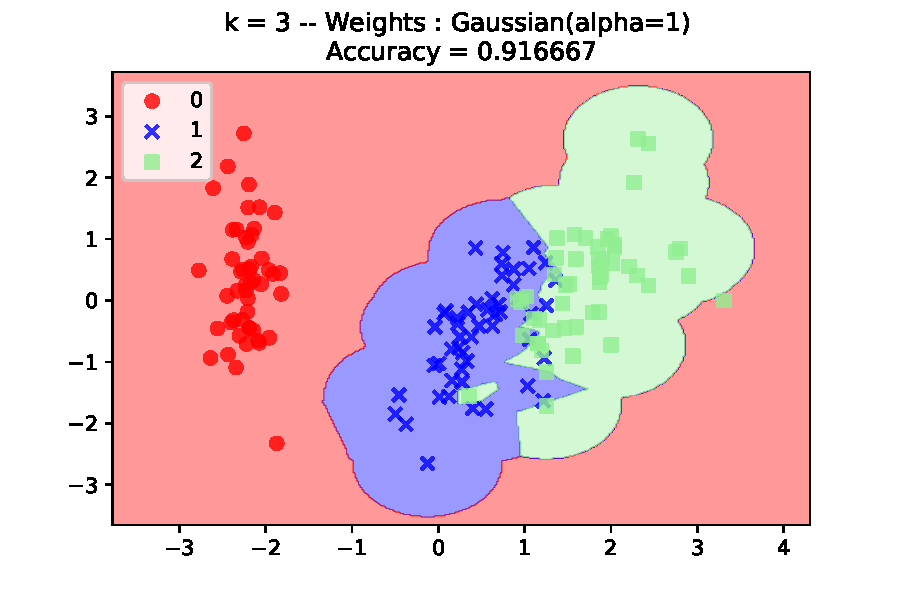
\includegraphics[width=0.7\linewidth]{../Images/Best_choice_Gaussian(alpha=1)}
		\caption{Best model with gaussian function.}
		\label{fig:Best_choice_Gaussian(alpha=1)}
		\end{figure}


	
\end{document}